\documentclass[russian,utf8,emptystyle]{eskdtext}

\newcommand{\No}{\textnumero} % костыль для фикса ошибки

\ESKDdepartment{Московский государственный технический университет им. Н. Э. Баумана}
\ESKDcompany{Кафедра ИУ5, Автоматизированные системы обработки информации и управления}
\ESKDclassCode{23 0102}
\ESKDtitle{Курсовая работа по дисциплине <<Супер ЭВМ>>}
\ESKDdocName{<<АИС о поставках малого предприятия>> (осуществление поставки малого предприятия)}
\ESKDauthor{Гуща~А.~В.}
\ESKDtitleApprovedBy{к.т.н. доцент}{Тоноян С.А.}
\ESKDtitleAgreedBy{к.т.н. доцент}{Тоноян С.А.}
\ESKDtitleDesignedBy{Студент группы ИУ5-92}{Гуща~А.~В}

\usepackage{multirow}
\usepackage{tabularx}
\usepackage{tabularx,ragged2e}
\usepackage{pdfpages}
\renewcommand\tabularxcolumn[1]{>{\Centering}p{#1}}
\newcommand\abs[1]{\left|#1\right|}

\usepackage{longtable,tabu}

\usepackage{geometry}
\geometry{footskip = 1cm}

\pagenumbering{arabic}
\pagestyle{plain}

\usepackage{setspace}
\usepackage{enumitem}

\usepackage{xcolor}
\usepackage{listings}
\lstset{
    breaklines=true,
    postbreak=\raisebox{0ex}[0ex][0ex]{\ensuremath{\color{red}\hookrightarrow\space}},
    extendedchars=\true,
    basicstyle=\small,
    inputencoding=utf8
}
\lstdefinelanguage{D}{
    keywords = {
    abstract,
    alias,
    align,
    asm,
    assert,
    auto,
    body,
    bool,
    break,
    byte,
    case,
    cast,
    catch,
    cdouble,
    cent,
    cfloat,
    char,
    class,
    const,
    continue,
    creal,
    dchar,
    debug,
    default,
    delegate,
    delete,
    deprecated,
    do,
    double,
    else,
    enum,
    export,
    extern,
    false,
    final,
    finally,
    float,
    for,
    foreach,
    foreach_reverse,
    function,
    goto,
    idouble,
    if,
    ifloat,
    immutable,
    import,
    in,
    inout,
    int,
    interface,
    invariant,
    ireal,
    is,
    lazy,
    long,
    macro,
    mixin,
    module,
    new,
    nothrow,
    null,
    out,
    override,
    package,
    pragma,
    private,
    protected,
    public,
    pure,
    real,
    ref,
    return,
    scope,
    shared,
    short,
    static,
    struct,
    super,
    switch,
    synchronized,
    template,
    this,
    throw,
    true, 
    try,
    typedef,
    typeid,
    typeof,
    ubyte,
    ucent,
    uint,
    ulong,
    union,
    unittest,
    ushort,
    version,
    void,
    volatile,
    wchar,
    while,
    with,
    __FILE__,
    __MODULE__,
    __LINE__,
    __FUNCTION__,
    __PRETTY_FUNCTION__,
    __gshared,
    __traits,
    __vector,
    __parameters,
    }
}

\begin{document}
\maketitle
%\includepdf[pages={1}]{title.pdf}

\tableofcontents
\clearpage

\section{Техническое задание}

29 вариант - <<АИС о поставках малого предприятия>>.

\subsection{Наименование}
Проектирование распределенной сети обработки информации АИС о поставках малого предприятия.

\subsection{Основание для разработки}
Основанием для разработки является учебный план кафедры ИУ5 МГТУ им. Н.Э. Баумана.

\subsection{Цель разработки}
Целью разработки является создание проектного решения на распределенную сеть обработки информации, объединяющуюю все отделы АИС малого предприятия, состоящей из центрального офиса и пяти отделов (дополнительных офисов).

\subsection{Задачи, подлежащие решению}
В процессе выполнения курсовой работы необходимо решить следующие задачи:
\begin{enumerate}[label=\arabic*)]
\item Запроектировать сеть по архитектуре клиент-сервер;
\item Для центрального офиса выбрать супер ЭВМ типа мейнфрейм и соответствующую операционную систему из линейнки z/OS. Выбор произвести используя методику анализа прототипов и аналогв (не менее 3-4 аналогов по 5-7 критериям). Задаться количетсвенными характеристиками для запросов для АИС;
\item Разработать модель бизнес процесса АИС в нотации BPMN в виде диаграмм. Привести словесное описание бизнес процесса. Диаграмма моделирования бизнес процесса в нотации BPMN должна содержать следующие элементы:
\begin{itemize}[label=-]
\item объекты потока управления;
\item соединяющие объекты;
\item роли (не менее 2 пулов или 1 пул и 2 дорожки).
\end{itemize}
\item В качестве СУБД выбрать DB2 для использования с <<1С: Предприятие 8>>. Обосновать выбор режимов архивации и восстановаления информационной БД.
\end{enumerate}

\subsection{Требования к составу технических средств}
В центральном офисе используется мейнфрейм производства корпорации IBM.

\subsection{Требования к составу программных средств}
Операционная система из линейки z/OS.

\subsection{Техническая документация, предъявляемая по окончанию работы}
По окончанию работы должна быть предъявлена следующая документация:
\begin{itemize}[label=-]
\item структурная схема спроектированной сети;
\item модель бизнес-процесса АИС в нотации BPMN;
\item схема спроектированной БД;
\item пояснительная записка.
\end{itemize}

\subsection{Порядок приема работы}
Прием работы осуществляется путем проверки соответствия выполненной работы пунктам технического задания.

\subsection{Дополнительные условия}
Данное техническое задание может уточняться в установленном порядке.

\clearpage
\section{Проектирование сети автоматизированной информационной системы}
\subsection{Обоснование выбора архитектуры клиент-сервер}

Архитектурой сети была выбрана клиент-серверная архитектура в соответствии с техническим заданием. 

\textbf{Клиент-сервер} - сетева архитектура или организация построения сети, в которой производится разделение вычислительной нагрузки между включенными в ее состав компьютерами, выполняющие функции клиентов, и одной мощной центральной ЭВМ - сервером.

Сервер может поддерживать центральную базу данных, расположенных на большом компьютере, зарезервированном для этой цели. \textbf{Клиент} - сторона (ЭВМ, программа или пользователь), запрашивающая и использующая информацию и/или ресурсы у сервера в среде клиент-сервер.

Достоинства архтектуры клиент-сервер:
\begin{itemize}[label=-]
\item отсутствие дублирования кода программы-сервера программами-клиентами;
\item требования к клиентским копьютерам снижаются, так как все вычисления выполняются на сервере;
\item лучшая защита данных, так как все данные хранятся на сервере и обеспечить надлежащую защиту сервера легче, чем всех клиентов. Также на сервере возможно разделение полномочий, позволяющее допускать клиентов к данным только с соответствующим уровнем доступа;
\item клиенты могут быть неоднородны по аппаратному и программному обеспечению;
\end{itemize}

Недостатки архитектуры клиент-сервер:
\begin{itemize}[label=-]
\item необходим очень мощный сервер, что означает большие финансовые затраты, которые зачастую не компенсируются удешевлением клиентских машин;
\item при недостаточной защите данных на сервере злоумышленник получает доступ ко всем ресурсам АИС;
\item отказ сервера приводит к отказу всей АИС;
\item плохая масштабируемость, при увеличении числа клиентов необходимо полностью менять аппаратуру сервера;
\item большая нагрузка на сеть, передача данных между клиентами и сервером занимают большую часть сетевых ресурсов сети;
\end{itemize}

\subsection{Схема сети АИС}

Схема сети, спроектированной для АИС, представлена на рисунке~\ref{fig:network}. Сеть АИС включает центральный офис и пять дополнительных офисов.

\begin{figure}[h!]
\centering
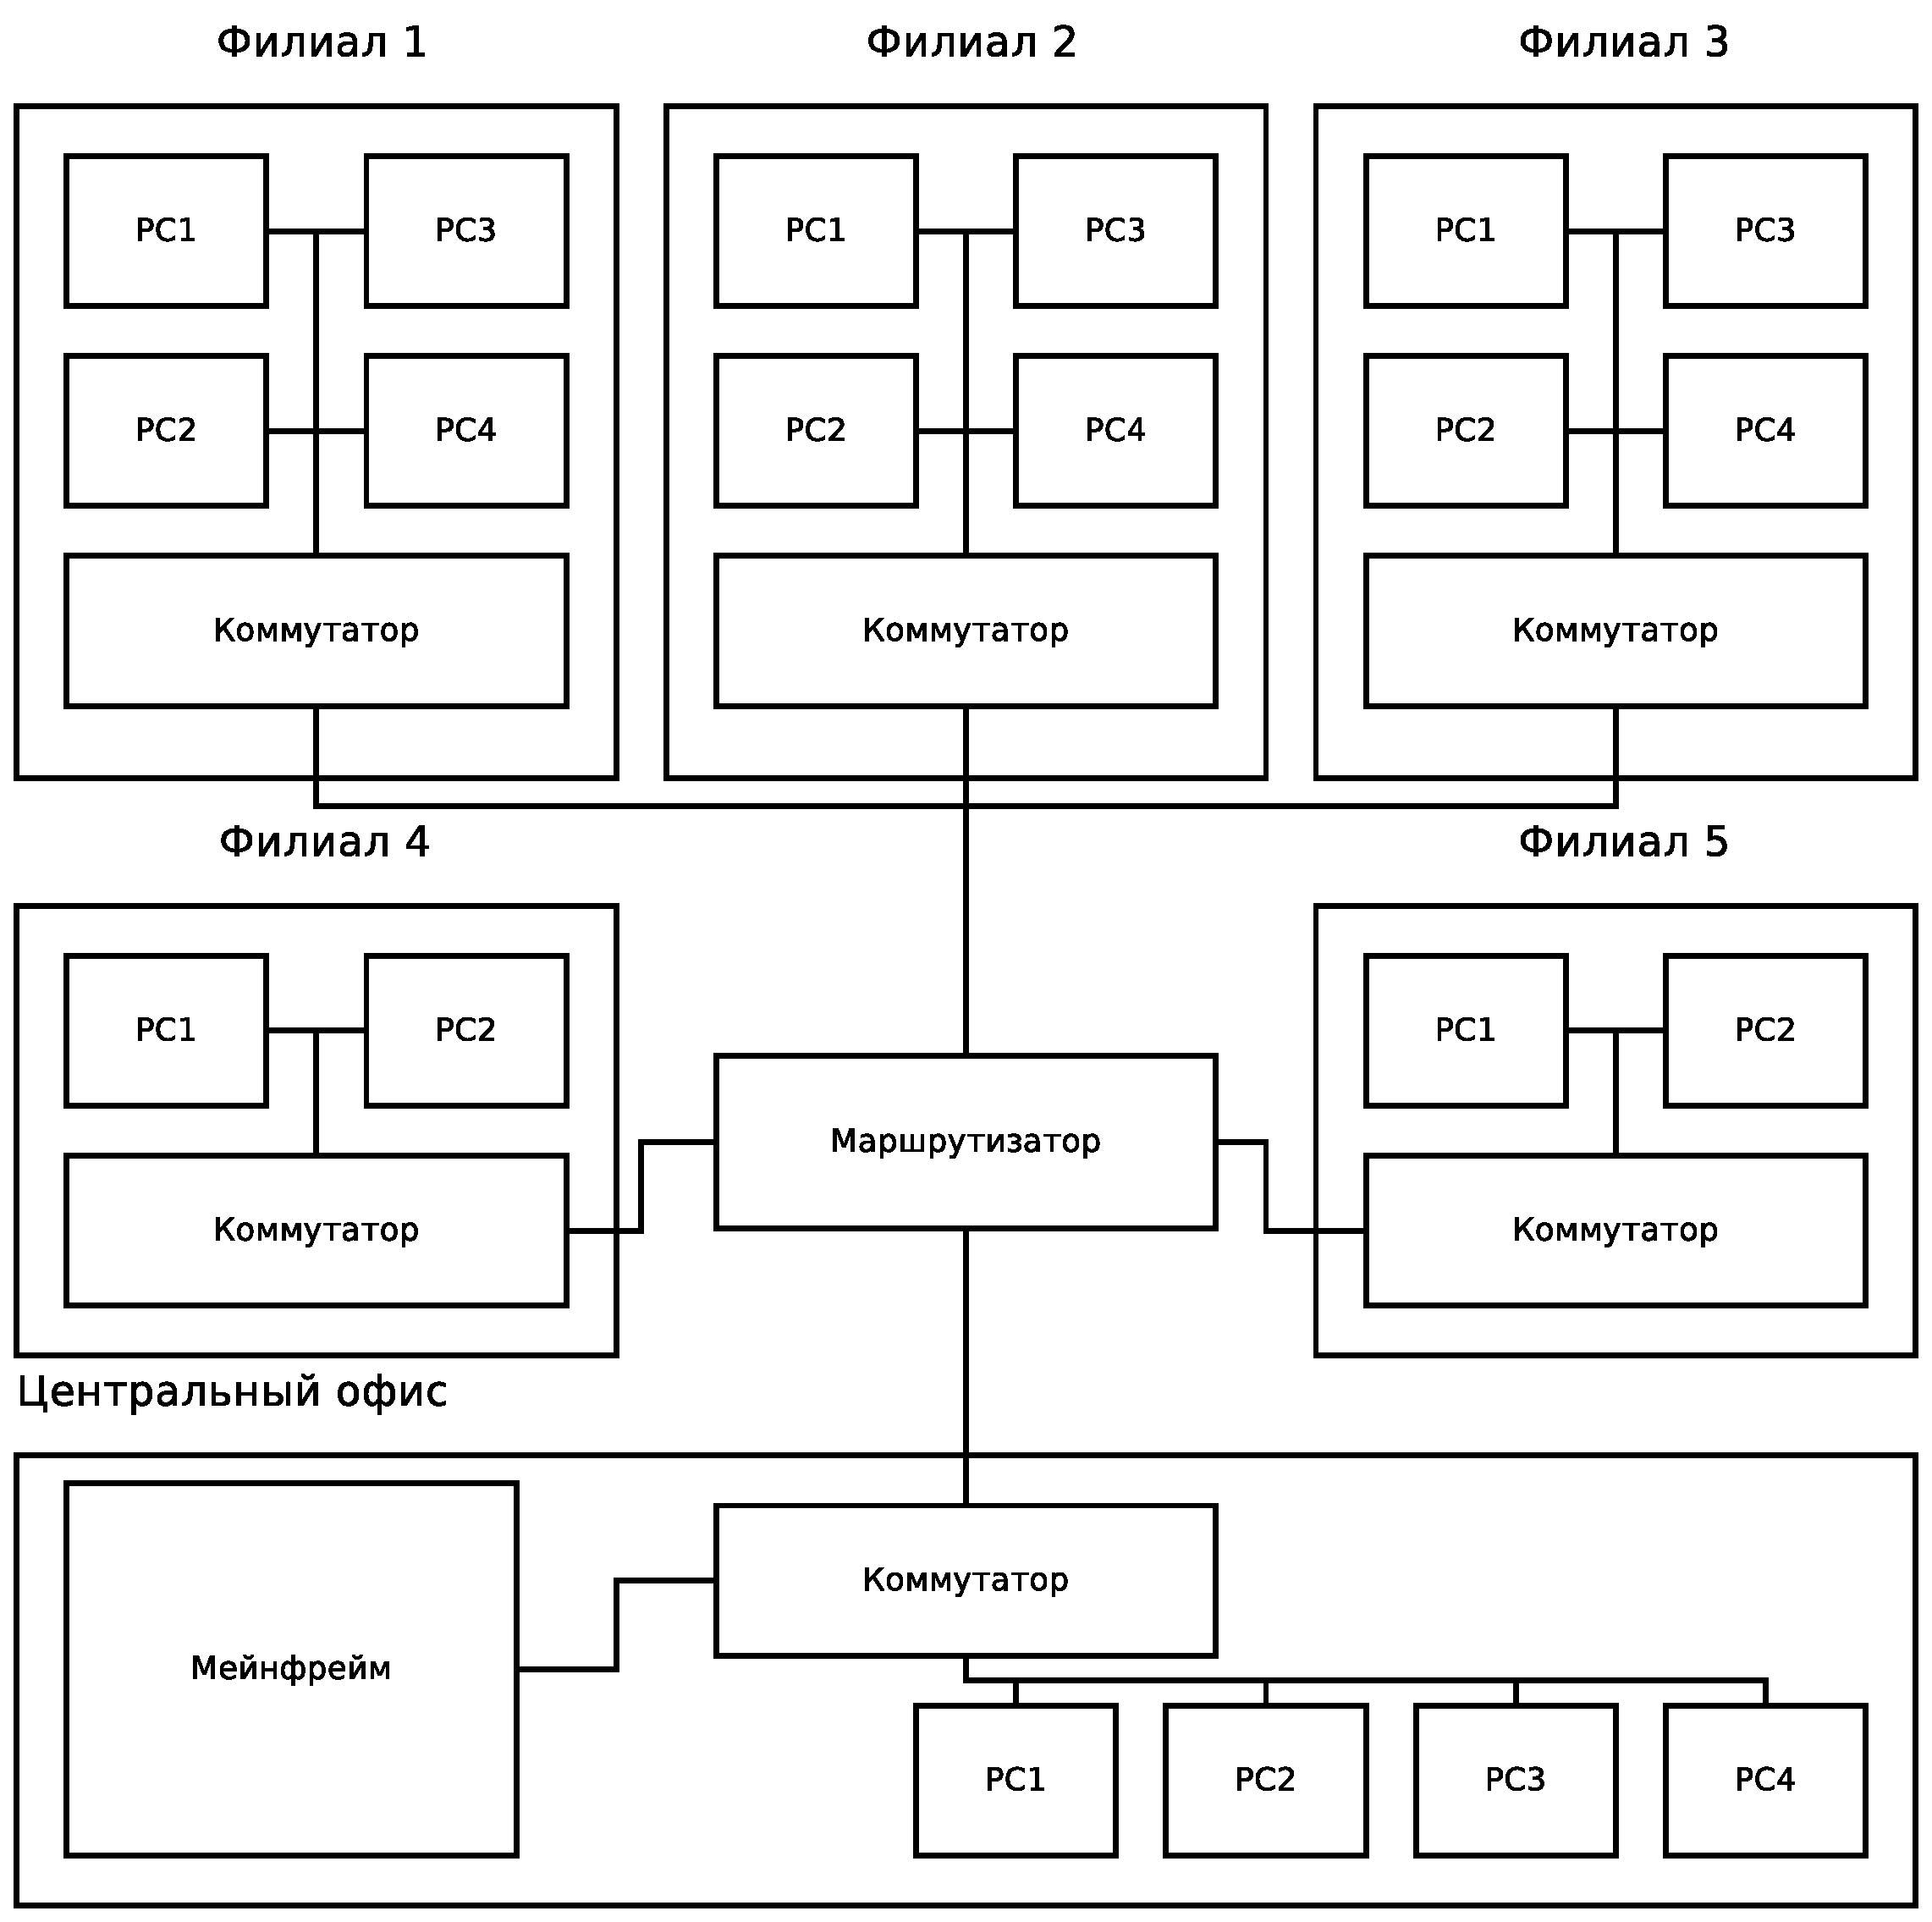
\includegraphics[width=0.8\textwidth]{network}
\caption{Схема сети АИС}
\label{fig:network}
\end{figure}

Сеть строится на базе технологии 100Base-TX, которая обладает следующими преимуществами:
\begin{itemize}[label=-]
\item распространненность, гарантированная поддержка широким классом оборудования;
\item высокая надежность;
\item низкая стоимость;
\item расстояние между узлами до 100 метров.
\end{itemize}

В главном офисе наряду с рабочими станциями устанавливается мэйнфрейм а также хранилища данных для БД и резервных копий.

\clearpage
\section{Выбор оборудования и операционной системы для офисов}
\subsection{Особенности и характеристики современных мейнфреймов}

\textbf{Мейнфрейм} — наиболее мощный высокопроизводительный компьютер со значительным объёмом оперативной и внешней, используемый в качестве главного или центрального компьютера.

На решение выбрать мейнфрейм в качестве супер ЭВМ повлиял ряд их преимуществ перед обычным ЭВМ:
\begin{enumerate}[label=-]
\item в мейнфреймах используется память с коррекцией ошибок. Ошибки не приводят к разрушению данных в памяти, или данных, ожидающих вывода на внешние устройства. Дисковые подсистемы построенные на основе RAID-массивов с горячей заменой и встроенных средств резервного копирования защищают от потерь данных;
\item рабочая нагрузка мейнфреймов может составлять 80-95\% от их пиковой производительности. Операционная система мейнфрейма будет обрабатывать всё сразу, причём все приложения будут тесно сотрудничать и использовать общие компоненты ПО;
\item подсистемы ввода-вывода мейнфреймов разработаны так, чтобы работать в среде с высочайшей рабочей нагрузкой на ввод-вывод данных;
\item мейнфреймы могут изолировать и исправлять большинство аппаратных и программных ошибок за счёт использования двух принципов:
\begin{enumerate}[label=-]
\item дублирование: два резервных процессора, резервные модули памяти, альтернативные пути доступа к периферийным устройствам;
\item горячая замена всех элементов вплоть до каналов, плат памяти и центральных процессоров;
\end{enumerate}
\item масштабирование мейнфреймов может быть как вертикальным, так и горизонтальным. Вертикальное масштабирование обеспечивается линейкой процессоров с производительностью от 5 до 200 MIPS и наращиванием до 12 центральных процессоров в одном компьютере. Горизонтальное масштабирование реализуется объединением ЭВМ в Sysplex (System Complex) — многомашинный кластер, выглядящий с точки зрения пользователя единым компьютером. Всего в Sysplex можно объединить до 32 машин. Программное масштабирование — на одном мейнфрейме может быть сконфигурировано фактически бесконечное число различных серверов. Причем все серверы могут быть изолированы друг от друга так, как будто они выполняются на отдельных выделенных компьютерах и в то же время совместно использовать аппаратные и программные ресурсы и данные;
\item поскольку данные хранятся на одном сервере, прикладные программы не нуждаются в сборе исходной информации из множества источников, не требуется дополнительное дисковое пространство для их временного хранения, не возникают сомнения в их актуальности;
\item встроенные в аппаратуру возможности защиты, такие как криптографические устройства и средства защиты операционных систем, дополненные программными продуктами RACF или VM:SECURE, обеспечивают надёжную защиту;
\item использование данных и существующих прикладных программ не влечёт дополнительных расходов по приобретению нового программного обеспечения для другой платформы, переподготовке персонала, переноса данных и т.д.
\item время наработки на отказ современных мейнфреймов оценивается в 12-15 лет;
\end{enumerate}

\subsection{Операционные системы из линейки z/OS}
\textbf{z/OS} — проприетарная 64-битная серверная операционная система, разработанная компанией IBM для мейнфреймов собственного производства. Является дальнейшим развитием операционной системы OS/390, объединяя MVS и системные службы Unix (POSIX-совместимая реализация для Unix, изначально известная как MVS OpenEdition или OpenMVS).

Содержит большинство функций, реализованных в 1970-х и 1960-х (в некоторых случаях), z/OS также предлагает многие отличительные черты и элементы, идентичные таковым в ныне доступных открытых системах. Таким образом, в то время как CICS, IMS, RACF, SNA и подобные функциональные возможности до сих пор продолжают ежедневно использоваться, они стали менее заметными, чем в прошлые годы.

На данный момент z/OS поддерживает Java, Unix API и приложения, и легко взаимодействует с TCP/IP и web. Сопутствующий продукт IBM, z/VM, улучшает поддержку Linux на той же самой системе. Поддержка действующих стандартов функциональности в z/OS и поддержка Linux и OpenSolaris позволяет наращивать возможности для будущего использования.

z/OS работает также на мейнфреймах более ранних архитектур, чем z/Architecture, которые работали в 32-битном режиме, и с аппаратным обеспечением, использующим 24-битную адресацию памяти. Тем не менее, начиная с версии z/OS V1R6, выпущенной 24 сентября 2004 года, z/OS требует 64-битные серверы IBM System z. Поддержка версии z/OS V1R5 осуществлялась до 31 марта 2007 года.

z/OS является передовой ОС, разрабатываемой IBM, предназначенной для продолжительной работы с большим количеством операций с высоким уровнем безопасности и устойчивости.

Диалоговое взаимодействие пользователя с ОС осуществляется через интерфейс ISPF.

\subsection{Выбор оборудования}
\textbf{IBM System z} — бренд, созданный компанией IBM для обозначения линейки мейнфреймов. Название «IBM System z» в настоящее время относится ко всем моделям, поддерживающим z/Architecture, то есть к семействам IBM zSeries, IBM System z9 и IBM System z10.

В 2000 году компания IBM на смену архитектуры IBM System/390 объявила новую 64-разрядную архитектуру IBM eServer zSeries, и уже в октябре 2000 была выпущена первая модель этого семейства zSeries 900. В 2002 году была представлена новая базовая модель zSeries 800; в апреле появился сервер zSeries 890.

В 2005 году на смену моделям zSeries было представлено семейство IBM System z9. Тогда же было введено название «IBM System z», объединяющее эти семейства. В 2008 году было представлено семейство IBM System z10, реализующее новый уровень архитектуры z/Architecture 2. И самые современные мейнфреймы IBM семейства zEnterprise были представленны 2010 году.

Модельный ряд:
\begin{itemize}[label=-]
\item IBM System z10 EC12 H20;
\item IBM System z10 EC13 H43;
\item IBM System z10 EC14 H66;
\item IBM System z10 EC15 H89;
\item IBM System z10 EC16 HA1.
\end{itemize}

Необходимо выбрать одну модель из линейки для спроектированной АИС. Проведем выбор методом сравнения прототипов и аналогов, количественные характиристики моделей представлены в таблице~\ref{tab:mainframe-1}.

\textbf{zApplication Assist Processor (zAAP)} - специализированный процессор для выполнения JAVA и XML приложений.

\textbf{System Assist Processor (SAPs)} - специализированный процессор для ускорения ввода-вывода.

\begin{longtable}{p{5cm}|p{1.5cm}|p{1.5cm}|p{1.5cm}|p{1.5cm}|p{1.5cm}}
\caption{Количественные характеристики моделей мейнфреймов семейства zEnterprise.}
\label{tab:mainframe-1} \\
Параметр                    & H20 & H43 & H66 & H89 & HA1 \\
\hline
Максимальное число ЦП       & 20  & 43  & 66  & 89  & 101 \\
Максимальное число zAAP     & 10  & 21  & 33  & 44  & 50 \\
Максимальное число SAPs     & 8   & 16  & 24  & 32  & 32 \\
Максимальная память ОП, Гб  & 704 &1392 &2272 &3040 &3040 \\
Стоимость, тысячи долларов  & 750 &1300 &1800 &2200 &2600 \\
\end{longtable}

Пронормализиуем параметры и распределим весовые коэффициенты, результаты представлены в таблице~\ref{tab:mainframe-2}.

\begin{longtable}{p{5cm}|p{1.5cm}|p{1.5cm}|p{1.5cm}|p{1.5cm}|p{1.5cm}|p{1.5cm}}
\caption{Нормализованные характеристики моделей мейнфреймов семейства zEnterprise.}
\label{tab:mainframe-2} \\
Параметр                    & $\alpha$ & H20 & H43 & H66 & H89 & HA1 \\
\hline
Максимальное число ЦП       & 0.2      & 0.2 & 0.43& 0.65& 0.88& 1.0 \\
Максимальное число zAAP     & 0.05     & 0.2 & 0.42& 0.66& 0.88& 1.0 \\
Максимальное число SAPs     & 0.05     & 0.25& 0.5 & 0.75& 1.0 & 1.0 \\
Максимальная память ОП, Гб  & 0.1      & 0.23& 0.46& 0.75& 1.0 & 1.0 \\
Стоимость, тысячи долларов  & 0.6      & 1.0 & 0.58& 0.42& 0.34& 0.29 \\
\hline
                            & 1.0      & 0.69& 0.53& 0.53& 0.57& 0.57 \\
\end{longtable}

Из таблицы видно, что следует предпочесть IBM System z10 EC16 H20.

\section{Модель бизнес процесса АИС}
\subsection{Нотация BPMN}
\textbf{BPMN (Business Process Model and Notation)} — система условных обозначений для моделирования бизнес-процессов. Разработана Business Process Management Initiative (BPMI) и поддерживается Object Management Group, после слияния организаций в 2005 году.

Спецификация BPMN описывает условные обозначения для отображения бизнес-процессов в виде диаграмм бизнес-процессов. BPMN ориентирована как на технических специалистов, так и на бизнес-пользователей. Для этого язык использует базовый набор интуитивно понятных элементов, которые позволяют определять сложные семантические конструкции.

Основная цель BPMN — создание стандартного набора условных обозначений, понятных всем бизнес-пользователям. Бизнес-пользователи включают в себя бизнес-аналитиков, создающих и улучшающих процессы, технических разработчиков, ответственных за реализацию процессов и менеджеров, следящих за процессами и управляющих ими. Следовательно, BPMN призвана служить связующим звеном между фазой дизайна бизнес-процесса и фазой его реализации.

В настоящий момент существует несколько конкурирующих стандартов для моделирования бизнес-процессов. Распространение BPMN поможет унифицировать способы представления базовых концепций бизнес-процессов, а также более сложные концепции.

BPMN поддерживает лишь набор концепций, необходимых для моделирования бизнес процессов. Моделирование иных аспектов, помимо бизнес процессов, находится вне зоны внимания BPMN.

Моделирование бизнес-процессов используется для донесения широкого спектра информации до различных категорий пользователей. Диаграммы бизнес-процессов позволяют описывать сквозные бизнес-процессы, но в то же время помогают читателям быстро понимать процесс и легко ориентироваться в его логике. В сквозной BPMN-модели можно выделить три типа подмоделей:
\begin{enumerate}[label=\arabic*)]
\item частные (внутренние) бизнес-процессы;
\item абстрактные (открытые) бизнес-процессы;
\item процессы взаимодействия (глобальные).
\end{enumerate}

Частные бизнес-процессы описывают внутреннюю деятельность организации. Они представляют бизнес-процессы в общепринятом. При использовании ролей частный бизнес-процесс помещается в отдельный пул. Поэтому поток управления находится внутри одного пула и не может пересекать его границ. Поток сообщений, напротив, пересекает границы пулов для отображения взаимодействия между разными частными бизнес-процессами.

Абстрактные (открытые) бизнес-процессы служат для отображения взаимодействия между двумя частным бизнес-процессами. В открытом бизнес процессе показываются только те действия, которые участвуют в коммуникации с другими процессами. Все другие, «внутренние», действия частного бизнес-процесса не показываются в абстрактном процессе. Абстрактные процессы помещаются в пулы и могут моделироваться как отдельно, так и внутри большей диаграммы бизнес-процессов для отображения потока сообщений между действиями абстрактного процесса с другими элементами.

Процесс взаимодействия (глобальный) отображает взаимодействия между двумя и более сущностями. Эти взаимодействия определяются последовательностью действий, обрабатывающих сообщений между участниками. Процессы взаимодействия могут помещаться в пул. Эти процессы могут моделироваться как отдельно, так и внутри большей диаграммы бизнес-процессов для отображения ассоциаций между действиями и другими сущностями.

\clearpage
\subsection{Диаграмма бизнес процесса в нотации BPMN}
Моделирование в BPMN осуществляется посредством диаграмм с небольшим числом графических элементов. Это помогает пользователям быстро понимать логику процесса. Выделяют четыре основные категории элементов:
\begin{enumerate}[label=\arabic*]
\item объекты потока управления: события, действия и логические операторы
\item соединяющие объекты: поток управления, поток сообщений и ассоциации
\item роли: пулы и дорожки
\item артефакты: данные, группы и текстовые аннотации.
\end{enumerate}

Элементы этих четырёх категорий позволяют строить простейшие диаграммы бизнес-процессов. Для повышения выразительности модели спецификация разрешает создавать новые типы объектов потока управления и артефактов.

Рассмотрим один процесс заданной предметной области – процесс осуществления поставки малого предприятия. Диаграмма бизнес процесса в нотации BPMN приведена на рисунке~\ref{fig:bpmn-1}.

\begin{figure}[h!]
\centering
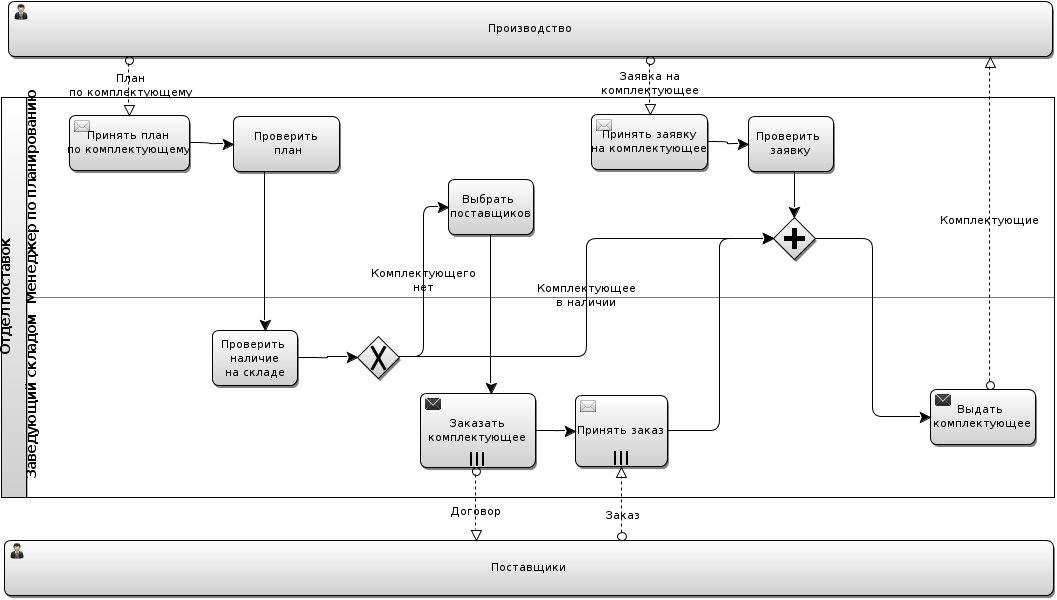
\includegraphics[width=0.9\textwidth]{superpc}
\caption{Процесс осуществления поставки малого предприятия}
\label{fig:bpmn-1}
\end{figure}

На предприятии выделяются два отдела - отдел производства и отдел планирования. Производство предварительно составляет план по комплектующим, которые будут использованы в текущем рассчетном периоде. Этот план отслывается отделу по планированию. План проверяется менеджером по планированию на непротиворечивость и соответствию принятым правилам, а заведующий по складу сразу проверяет наличие данного комплектующего на складе. Если комплектующего нет в нужном объеме, то менеджер по планированию выбирает множество заказчиков, у которых будет закуплено комплектующее. Заведующий складом оформляет договоры на покупку и поставку, а также заведует процессом приемки заказа. 

Как только производству необходимо комплектующее из плана, менеджеру по планированию отсылается заявка, которую он проверяет и отдает заведующему склада. Заведующий складом отсылает комплектующие в нужном объеме на производство.

\clearpage
\section{Выбор СУБД DB2 для использования с 1С: Предприятие 8}
\subsection{Система управления базами данных DB2}

В качестве СУБД выберем DB2 - семейство систем управления реляционными базами данных, выпускаемых корпорацией IBM.

Диалект языка SQL, используемый в DB2 за редкими исключениями строго декларативен, система снабжена многофазовым оптимизатором, строящий по этим декларативным конструкциям план выполнения запроса. В диалекте SQL DB2 практически отсутствуют подсказки оптимизатору, мало развит язык хранимых процедур, и, таким образом, всё направлено на поддержание декларативного стиля написания запросов. Язык SQL DB2 при этом является вычислительно полным, то есть потенциально позволяет в декларативной форме определять любые вычислимые соответствия между исходными данными и результатом. Это достигается в том числе за счёт использования табличных выражений, рекурсии и других развитых механизмов манипулирования данными.

DB2 является единственной реляционной СУБД общего назначения, имеющей реализации на аппаратно-программном уровне. В оборудовании мэйнфреймов IBM System z реализуются средства поддержки DB2.

1С:Предприятие — программный продукт компании 1С, предназначенный для автоматизации деятельности на предприятии. 1С:Предприятие — это и технологическая платформа, и пользовательский режим работы. Технологическая платформа предоставляет объекты и механизмы управления объектами. Объекты (данные и метаданные) описываются в виде конфигураций. При автоматизации какой-либо деятельности составляется своя конфигурация объектов, которая и представляет собой законченное прикладное решение. Конфигурация создаётся в специальном режиме работы программного продукта под названием «Конфигуратор», затем запускается режим работы под названием «1С:Предприятие», в котором пользователь получает доступ к основным функциям, реализованным в данном прикладном решении (конфигурации).

Технологическая платформа «1С:Предприятие» представляет собой программную оболочку над базой данных. Кроме того, с версии 8.1 хранение данных возможно в СУБД PostgreSQL и IBM DB2, а с версии 8.2 добавилась и Oracle. Имеет свой внутренний язык программирования, обеспечивающий, помимо доступа к данным, возможность взаимодействия с другими программами.

\subsection{Режимы архивации и резервного копирования информационной БД}
Резервное копирование (англ. backup) — процесс создания копии данных на носителе (жёстком диске, дискете и т.д.), предназначенном для восстановления данных в оригинальном или новом месте их расположения в случае их повреждения или разрушения.


\end{document}